\documentclass[fontsize=14pt,DIV=1,a4paper]{scrartcl} 
\usepackage[utf8]{inputenc}
\usepackage{cmap} % для кодировки шрифтов в pdf
\usepackage[T2A]{fontenc}
%\usepackage{fontspec}
%\usepackage{polyglossia}
%\setmainfont{Times New Roman}
%\newfontfamily\cyrillicfont{Times New Roman}
%\usepackage{mathptmx}
%\renewcommand{\rmdefault}{ftm} % Times New Roman
\linespread{1.3} % полуторный интервал
\frenchspacing
\usepackage[english,russian,ukrainian]{babel}
\usepackage{indentfirst}
\usepackage{misccorr}
\usepackage{graphicx}
\usepackage[left=3cm,right=1.5cm,top=2cm,bottom=2cm,includefoot]{geometry}
\usepackage{graphicx}% для вставки картинок
\graphicspath{ {/home/zeka/Documents/lab2chmmph/} }

\usepackage{amssymb,amsfonts,amsmath,amsthm} % математические дополнения от АМС
\usepackage{indentfirst} % отделять первую строку раздела абзацным отступом тоже
\usepackage[usenames,dvipsnames]{color} % названия цветов
\usepackage{makecell}
\usepackage{multirow} % улучшенное форматирование таблиц
\usepackage{ulem} % подчеркивания
\usepackage{gensymb}
\usepackage{hyperref}
\hypersetup{
    colorlinks=true,
    linkcolor=black,
    filecolor=black,      
    urlcolor=black,
}

\makeatletter
\DeclareOldFontCommand{\rm}{\normalfont\rmfamily}{\mathrm}
\DeclareOldFontCommand{\sf}{\normalfont\sffamily}{\mathsf}
\DeclareOldFontCommand{\tt}{\normalfont\ttfamily}{\mathtt}
\DeclareOldFontCommand{\bf}{\normalfont\bfseries}{\mathbf}
\DeclareOldFontCommand{\it}{\normalfont\itshape}{\mathit}
\DeclareOldFontCommand{\sl}{\normalfont\slshape}{\@nomath\sl}
\DeclareOldFontCommand{\sc}{\normalfont\scshape}{\@nomath\sc}
\makeatother

\begin{document}
	\begin{titlepage}
		\begin{center}
			\large
			\textbf{КИЇВСЬКИЙ НАЦІОНАЛЬНИЙ УНІВЕРСИТЕТ \\
			ІМЕНІ ТАРАСА ШЕВЧЕНКА}

			\textbf{Кафедра обчислювальної математики}
			
			\vspace{6.0cm}

			\textsc{Лабораторна робота 3}\\
			На тему:

			\textbf{ Вирішення задач теплопровідності }
			\bigskip
		\end{center}
		\vfill

		\hfill
		\begin{minipage}{0.6\textwidth}
			студента 4-го курсу бакалаврату\\
			Гаврилка Євгенія Дмитровича
		\end{minipage}%
		\vfill
		
		\vspace{-2.5cm}
		
		

		\vspace{1.0cm}

		\begin{center}
			Київ – 2017
		\end{center}
	\end{titlepage}
	
	%\tableofcontents

	%summary
	\newpage
	\addcontentsline{toc}{section}{Постанова задачі}
	\section*{Постанова задачі}
	Визначити температуру всередині і на повурхні цегляної колони діметром 0.5 м через одну годину, якщо раптово температура навколишнього середовища знизилась з +20 до - 20 С. Фізичні характеристики цегляної колони мають такі значення: $\lambda = 0.77\quad W/(m \cdot K); c= 0.83\quad kJ/(kg \cdot K); \rho = 1600 \quad kg/m^3ну ; \gamma = 7 \quad W/(m^2 \cdot K) $
	
	%section1
	\newpage
	\section{Метод безпосередньої заміни похідних частковими}
	\subsection{Теорія}
	Робимо заміну для обезрозміреного рівняння
	\begin{equation}
		\frac{\partial v}{\partial x_1} \Bigr|_{\substack{x_1=0}} = 0 
	\end{equation}
	\begin{equation}
		v'_0 = \frac{4v_1-v_2-3v_0}{2h} + O(h^2)
	\end{equation}
	\begin{equation}
		-3v_0+4v_1-v_2=0 
	\end{equation}
	
	\begin{equation}
		\frac{\partial v}{\partial x_1} + \gamma_1 \cdot v \Bigr|_{\substack{x_1=1}}= 0 
	\end{equation}
	\begin{equation}
		v'_N = \frac{v_N+3v_{N-1}-4v_{N-2}}{2h} + O(h^2)
	\end{equation}
	\begin{equation}
		v_{N-2}-4v_{N-1}+3v_N=-2\gamma_1\cdot h\cdot v 
	\end{equation}
	
	\newpage
	\begin{equation}
		\frac{u^{j+1}_i-u^j_i}{\tau} = (\frac{1}{x}(x(\sigma \cdot u^{j+1}+(1-\sigma) \cdot u^j)_{\bar{x}})_x)_i
	\end{equation}
	\begin{equation}
		x_i(u^{j+1}_i-u^j_i) = \frac{\tau}{h}(x_{i+0.5}(\sigma \cdot u^{j+1}+(1-\sigma) \cdot u^j)_{\bar{x},i+1} - x_{i-0.5}(\sigma \cdot u^{j+1}+(1-\sigma) \cdot u^j)_{\bar{x},i})
	\end{equation}
	
	\begin{equation}
		x_i(u^{j+1}_i-u^j_i) = \frac{\tau}{h^2}(
		  x_{i+0.5}(\sigma \cdot (u^{j+1}_{i+1}-u^{j+1}_{i})  +(1-\sigma) \cdot (u^j_{i+1}-u^{j}_{i}))
	\end{equation}
	\begin{equation}
		- x_{i-0.5}(\sigma \cdot (u^{j+1}_i    -u^{j+1}_{i-1})+(1-\sigma) \cdot (u^j_i-u^j_{i-1})
		)
	\end{equation}
	
	\begin{equation}
		x_i \cdot u^{j+1}_i - \frac{\tau}{h^2}(
		  x_{i+0.5}\cdot\sigma \cdot (u^{j+1}_{i+1}-u^{j+1}_{i})
		- x_{i-0.5}\cdot\sigma \cdot (u^{j+1}_i    -u^{j+1}_{i-1}))=
	\end{equation}
	\begin{equation}
		x_i \cdot u^j_i - \frac{\tau}{h^2}(
		  x_{i+0.5}\cdot(1- \sigma) \cdot (u^{j}_{i+1}-u^{j}_{i})
		- x_{i-0.5}\cdot(1- \sigma) \cdot (u^{j}_i    -u^{j}_{i-1}))
	\end{equation}
	
	\begin{equation}
		x_i \cdot u^{j+1}_i - \frac{\tau}{h^2}(
		  x_{i+0.5}\cdot\sigma \cdot (u^{j+1}_{i+1}-u^{j+1}_{i})
		- x_{i-0.5}\cdot\sigma \cdot (u^{j+1}_i    -u^{j+1}_{i-1}))=
	\end{equation}
	\begin{equation}
		x_i \cdot u^j_i - \frac{\tau}{h^2}(
		  x_{i+0.5}\cdot(1- \sigma) \cdot (u^{j}_{i+1}-u^{j}_{i})
		- x_{i-0.5}\cdot(1- \sigma) \cdot (u^{j}_i    -u^{j}_{i-1}))
	\end{equation}
	
	\begin{equation}
		- \frac{\tau}{h^2}\cdot x_{i-0.5}\cdot\sigma \cdot u_{i-1}
		+(x_i+\frac{\tau}{h^2}\cdot \sigma \cdot (x_{i-0.5}+x_{i+0.5}))\cdot u_i
		- \frac{\tau}{h^2}\cdot x_{i+0.5}\cdot\sigma \cdot u_{i+1}=
	\end{equation}
	\begin{equation}
		x_i \cdot u^j_i - \frac{\tau}{h^2}(
		  x_{i+0.5}\cdot(1- \sigma) \cdot (u^{j}_{i+1}-u^{j}_{i})
		- x_{i-0.5}\cdot(1- \sigma) \cdot (u^{j}_i    -u^{j}_{i-1}))
	\end{equation}
			
	\newpage
	\subsection{Алгоритм}
	Фізичні змінні:
	
	\begin{equation}
		u_1 = 20. + 273.15
	\end{equation}
	\begin{equation}
		u_0 = -20. + 273.15
	\end{equation}
	\begin{equation}
		\lambda = 0.77
	\end{equation}
	\begin{equation}
		c = 830.
	\end{equation}
	\begin{equation}
		\rho = 1600.
	\end{equation}
	\begin{equation}
		\gamma = 7.
	\end{equation}
	\begin{equation}
		R = 0.5
	\end{equation}
	\begin{equation}
		T = 3600
	\end{equation}
	
	Перехід до обезрозмірених змінних:
	
	\begin{equation}
		T_1 = \lambda / (c \cdot \rho \cdot R^2) \cdot T
	\end{equation}
	\begin{equation}
		\gamma_1 = R / \lambda \cdot \gamma
	\end{equation}
	
	Параметри різнецевої схеми:
	\begin{equation}
		N = 20
	\end{equation}
	\begin{equation}
		M = 20
	\end{equation}
	\begin{equation}
		\tau = T_1/M
	\end{equation}
	\begin{equation}
		h = 1 / N
	\end{equation}
	
	Різнецева схема:
	\begin{equation}
		A_{i,i-1} = -\sigma \cdot \tau / h^2 \cdot x_{i-0.5}
	\end{equation}
	\begin{equation}
		A_{i,i+1} = -\sigma \cdot \tau / h^2 \cdot x_{i+0.5}
	\end{equation}
	\begin{equation}
		A_{i,i} = x_i - A_{i,i-1} - A_{i,i+1}
	\end{equation}
	\begin{equation}
		\varphi_i = x_i \cdot y_i + \tau \cdot (1-\sigma)/h^2 \cdot (x_{i+0.5} \cdot (y_{i+1}-y_i)-x_{i-0.5} \cdot (y_i-y_{i-1}))
	\end{equation}
	
	Ліві крайові умови:
	\begin{equation}
		A_{0,0}=-3
	\end{equation}
	\begin{equation}
		A_{0,1}=4
	\end{equation}
	\begin{equation}
		A_{0,2}=-1
	\end{equation}
	\begin{equation}
		\varphi_{0}=0
	\end{equation}
	
	Праві крайові умови
	\begin{equation}
		A_{N, N}=3+2 \cdot h\cdot \gamma_1
	\end{equation}
	\begin{equation}
		A_{N, N-1}=-4
	\end{equation}
	\begin{equation}
		A_{N, N-2}=1
	\end{equation}
	\begin{equation}
		\varphi_{N}=0
	\end{equation}
	
	СЛАР:
	\begin{equation}
		A \cdot y = \varphi
	\end{equation}
	
	Повторюємо кроки 15-27 $M$ разів.
	
	\newpage
	\section{Iнтего-інтерполяційним метод}
	\subsection{Теорія}
	Розглядається задача Au=f з крайовими умовами. Головна ідея полягає в тому що б протабулювати значення функції на сітці. Крайові рівняння обирається так, щоб задовольняти крайовим умовам. Тобто
	\begin{figure}[h!]
		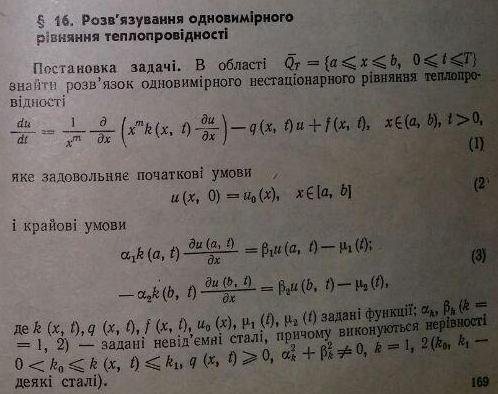
\includegraphics[scale=1.25]{th_ii1.jpg}
		\centering
		\caption{Теорія}
	\end{figure}
	
	\begin{figure}[h!]
		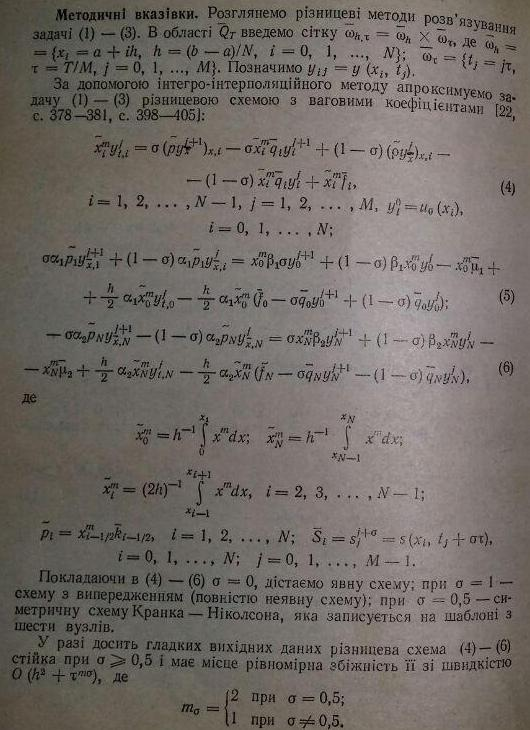
\includegraphics[scale=1.1]{th_ii2.jpg}
		\centering
		\caption{Теорія}
	\end{figure}
	
	\begin{figure}[h!]
		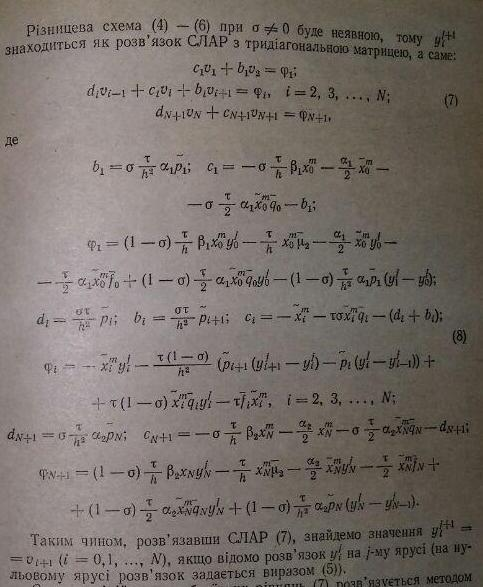
\includegraphics[scale=1.3]{th_ii3.jpg}
		\centering
		\caption{Теорія}
	\end{figure}
	
	\newpage
	\textbf{}
			
	\newpage
	\subsection{Алгоритм}
	
	\begin{figure}[h!]
		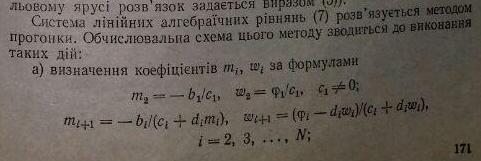
\includegraphics[scale=1.25]{algo_ii1.jpg}
		\centering
		\caption{Алгоритм}
	\end{figure}
	\begin{figure}[h!]
		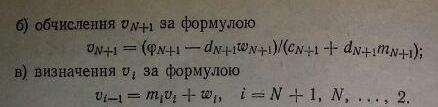
\includegraphics[scale=1.4]{algo_ii2.jpg}
		\centering
		\caption{Алгоритм}
	\end{figure}
	
	\newpage
	\section{Практична частина}

	\vspace{10px}
    n = 10, m = 20, t = 24h
    \vspace{10px}

    \begin{tabular}{c c c c c c c c c c c}
	  20.00&  20.00&  20.00&  20.00&  20.00&  20.00&  20.00&  20.00&  20.00&  20.00&  20.00 \\
	  20.00&  20.00&  20.00&  20.00&  19.99&  19.97&  19.91&  19.70&  18.97&  16.40&   7.27 \\
	  20.00&  20.00&  19.99&  19.98&  19.94&  19.82&  19.48&  18.56&  16.19&  10.82&   2.27 \\
	  19.99&  19.98&  19.96&  19.90&  19.75&  19.38&  18.52&  16.67&  13.09&   7.40&  -0.43 \\
	  19.94&  19.92&  19.85&  19.70&  19.35&  18.61&  17.18&  14.63&  10.58&   4.84&  -2.41 \\
	  19.83&  19.78&  19.64&  19.33&  18.72&  17.61&  15.71&  12.73&   8.44&   2.82&  -3.93 \\
	  19.61&  19.53&  19.29&  18.80&  17.93&  16.48&  14.23&  10.98&   6.61&   1.16&  -5.16 \\
	  19.25&  19.13&  18.79&  18.12&  17.01&  15.29&  12.80&   9.39&   5.01&  -0.25&  -6.19 \\
	  18.75&  18.60&  18.15&  17.33&  16.02&  14.09&  11.42&   7.93&   3.60&  -1.47&  -7.07 \\
	  18.12&  17.94&  17.41&  16.45&  14.98&  12.90&  10.11&   6.59&   2.34&  -2.54&  -7.84 \\
	  17.38&  17.18&  16.57&  15.50&  13.91&  11.72&   8.87&   5.35&   1.20&  -3.49&  -8.52 \\
	  16.55&  16.33&  15.66&  14.52&  12.84&  10.57&   7.70&   4.21&   0.16&  -4.34&  -9.13 \\
	  15.65&  15.41&  14.70&  13.50&  11.76&   9.46&   6.58&   3.15&  -0.79&  -5.11&  -9.68 \\
	  14.69&  14.45&  13.71&  12.47&  10.70&   8.38&   5.52&   2.15&  -1.66&  -5.82& -10.18 \\
	  13.71&  13.45&  12.70&  11.44&   9.65&   7.34&   4.52&   1.22&  -2.48&  -6.47& -10.64 \\
	  12.70&  12.44&  11.68&  10.41&   8.62&   6.33&   3.55&   0.34&  -3.23&  -7.08& -11.07 \\
	  11.68&  11.42&  10.66&   9.39&   7.62&   5.36&   2.64&  -0.49&  -3.94&  -7.64& -11.46 \\
	  10.66&  10.41&   9.65&   8.39&   6.64&   4.42&   1.76&  -1.27&  -4.61&  -8.16& -11.83 \\
	   9.65&   9.40&   8.65&   7.40&   5.68&   3.51&   0.93&  -2.01&  -5.24&  -8.66& -12.17 \\
	   8.65&   8.40&   7.66&   6.44&   4.76&   2.64&   0.13&  -2.72&  -5.83&  -9.12& -12.49 \\
	   7.67&   7.42&   6.70&   5.50&   3.86&   1.80&  -0.64&  -3.40&  -6.40&  -9.56& -12.80 \\
    \end{tabular}
	
	\newpage
	
    \vspace{10px}
    n = 10, m = 10, t = 1h
    \vspace{10px}

    \begin{tabular}{c c c c c c c c c c c}
	  20.00&  20.00&  20.00&  20.00&  20.00&  20.00&  20.00&  20.00&  20.00&  20.00&  20.00 \\
	  20.00&  20.00&  20.00&  20.00&  20.00&  20.00&  20.00&  20.00&  19.98&  19.60&  10.30 \\
	  20.00&  20.00&  20.00&  20.00&  20.00&  20.00&  20.00&  20.00&  19.92&  18.84&   9.53 \\
	  20.00&  20.00&  20.00&  20.00&  20.00&  20.00&  20.00&  19.99&  19.81&  18.13&   8.83 \\
	  20.00&  20.00&  20.00&  20.00&  20.00&  20.00&  20.00&  19.97&  19.66&  17.47&   8.19 \\
	  20.00&  20.00&  20.00&  20.00&  20.00&  20.00&  19.99&  19.93&  19.47&  16.84&   7.60 \\
	  20.00&  20.00&  20.00&  20.00&  20.00&  20.00&  19.99&  19.89&  19.27&  16.25&   7.05 \\
	  20.00&  20.00&  20.00&  20.00&  20.00&  20.00&  19.98&  19.84&  19.04&  15.69&   6.53 \\
	  20.00&  20.00&  20.00&  20.00&  20.00&  20.00&  19.96&  19.77&  18.80&  15.16&   6.05 \\
	  20.00&  20.00&  20.00&  20.00&  20.00&  19.99&  19.95&  19.69&  18.55&  14.66&   5.60 \\
	  20.00&  20.00&  20.00&  20.00&  20.00&  19.99&  19.93&  19.61&  18.29&  14.18&   5.18 \\
    \end{tabular}
	
	%results
	\newpage
	\addcontentsline{toc}{section}{Висновки}
	\section*{Висновки}
	
	Процес проходить досить природньо для цегли. Методичка по інтегро-інтерполяційному методу - жах.

\end{document}
